\documentclass[12pt,a4paper]{article}
\usepackage[utf8x]{inputenc}
\usepackage{ucs}
\usepackage{amsmath}
\usepackage{amsfonts}
\usepackage{amssymb}
\usepackage{graphicx}
\usepackage{grffile}
\usepackage{float}
\usepackage[portuguese]{babel}
\title{Trabalho 2}
\author{André Garnier Coutinho}
\setlength{\textwidth}{17cm}
\setlength{\textheight}{24cm}
\addtolength{\topmargin}{-2cm}
\addtolength{\oddsidemargin}{-2cm}
\begin{document}
\begin{center}
\textbf{Instituto de Matemática e Estatística da USP\linebreak MAT 2455 - Cálculo Diferencial e Integral III para Engenharia\linebreak Trabalho 2 - 1º semestre de 2015}
\end{center}

%%%%%%%%%%%%%%%%%%%%%%%%%%%%%%%%%%%%% Questão 1 %%%%%%%%%%%%%%%%%%%%%%%%%%%%%%%%%%%%%%%%%%%%%%%%

\textbf{Quest\~{a}o 1.} (2 pontos) Calcule a massa do sólido que ocupa a região interior ao elipsóide $x^2 + \frac{y^ 2}{4} + z^2 = 2z$ e tal que $z^2 \leq 3(x^2 + \frac{y^2}{4})$, $z \geq 0$, cuja densidade é $\delta(x,y,z) = x^2$. \\

\textbf{Solução:}
\linebreak
Devemos calcular a integral
\begin{equation}
 \iiint_{D_{xyz}}{x^2}\;dx\,dy\,dz \
\label{eq:integral}
\end{equation}

\begin{figure}[h!]
	\centering
	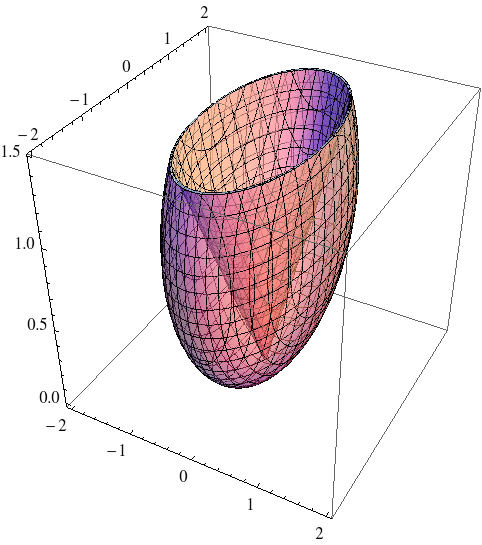
\includegraphics[scale=0.3]{Fig1.png}  
	\caption{Regi\~{a}o $ D_{xyz} = \lbrace(x, y, z)\mid x^2 + \frac{y^ 2}{4} + z^2 \leq 2z $, $z^2 \leq 3(x^2 + \frac{y^2}{4}) $ e $ z \geq 0 \rbrace $}
	\label{fig:figura1}
\end{figure}

Realizamos a seguinte mudança de coordenadas:
\begin{equation}
\left\{\begin{array}{ll}
x=\rho\sin\phi\,\cos\theta\\
y= 2\rho\sin\phi\,\sin\theta\\
z = \rho\cos\phi
\end{array}\right.
\label{eq:Q1_mudanca}
\end{equation}

\begin{equation}
J = \begin{Vmatrix}
\sin\phi\,\cos\theta &  \rho\cos\phi\,\cos\theta & -\rho\sin\phi\,\sin\theta \\
2\sin\phi\,\sin\theta & 2\rho\cos\phi\,\sin\theta & 2\rho\sin\phi\,\cos\theta \\
\cos\phi & -\rho\sin\phi & 0 \\
\end{Vmatrix} = 2\rho^2\sin\phi
\label{eq:Q1_Jac}
\end{equation}

Aplicando \eqref{eq:Q1_mudanca} \`a equaç\~{a}o do elipsóide:
\begin{equation}
\rho^2 = 2\rho\cos\phi \therefore \rho = 2\cos\phi
\label{eq:Q1_elipsoide}
\end{equation}

Aplicando \eqref{eq:Q1_mudanca} \`a equaç\~{a}o do cone elíptico :
\begin{equation}
\rho^2\cos^2\phi = 3 \rho^ 2 \sin^2\phi \Rightarrow \tan^2 \phi = \frac{1}{3} \therefore \phi = \frac{\pi}{6}
\label{eq:Q1_cone}
\end{equation}

Assim podemos facilmente descrever $D$ em coordenadas esf\'{e}ricas. \\

Calculando a integral : \

$$ \iiint_{D_{xyz}}{x^2}\;dx\,dy\,dz  = \int\limits_{0}^{2\pi} \int\limits_{\frac{\pi}{6}}^{\frac{\pi}{2}}  \int\limits_{0}^{2\cos\phi} \rho^2 \sin^2\phi\,\cos^2\theta \cdot 2 \rho^2 \sin\phi \;d\rho\, d\phi\,d\theta $$

$$ = 2\int\limits_{0}^{2\pi} \int\limits_{\frac{\pi}{6}}^{\frac{\pi}{2}}  \frac{\rho^5}{5} \Big|_{0}^{2\cos\phi} \sin^3\phi\,\cos^2\theta \;d\phi\,d\theta = \frac{2^6}{5} \int\limits_{0}^{2\pi} \int\limits_{\frac{\pi}{6}}^{\frac{\pi}{2}}  \cos^5\phi \sin^3\phi\,\cos^2\theta \;d\phi\,d\theta  $$
$$ = \frac{2^6}{5} \int\limits_{0}^{2\pi} \int\limits_{\frac{\pi}{6}}^{\frac{\pi}{2}}  \cos^5\phi (1 - \cos^2\phi) \sin\phi\,\cos^2\theta \;d\phi\,d\theta $$

Fazendo a seguinte mudaça de variável: $u = \cos\phi \Rightarrow du = -\sin\phi \, d\phi $, temos:

$$ = -\frac{2^6}{5} \int\limits_{0}^{2\pi} \int\limits_{\frac{\sqrt{3}}{2}}^{0}  u^5 (1 - u^2) \cos^2\theta \;du\,d\theta = \frac{2^6}{5} \int\limits_{0}^{2\pi} \int\limits_{0}^{\frac{\sqrt{3}}{2}}  u^5 (1 - u^2) \cos^2\theta \;du\,d\theta $$
$$ = \frac{2^6}{5} \int\limits_{0}^{2\pi}  \Big( \frac{u^6}{6} - \frac{u^8}{8} \Big)_{0}^{\frac{\sqrt{3}}{2}} \cos^2\theta \;d\theta = \frac{63}{160} \int\limits_{0}^{2\pi} \cos^2\theta \;d\theta $$
$$ = \frac{63}{160} \int\limits_{0}^{2\pi} \frac{1+\cos 2\theta}{2}  \; d\theta = \frac{63}{2\cdot 160} \Big( \theta + \frac{\sin 2\theta}{2} \Big)_{0}^{2\pi} = \frac{63 \pi}{160} $$

\newpage

%%%%%%%%%%%%%%%%%%%%%%%%%%%%%%%%%%%%% Questão 2 %%%%%%%%%%%%%%%%%%%%%%%%%%%%%%%%%%%%%%%%%%%%%%%%

\textbf{Quest\~{a}o 2.} (2 pontos) Calcule o volume do sólido limitado por $x^2 + y^2 = 1 + z^2$ e $x^2 + y^2 = 5$, isto é, $x^2 + y^2 \geq 1 + z^2$ e $x^2 + y^2 \leq 5$. \\

\textbf{Solução:}
\linebreak
Devemos calcular a integral
\begin{equation}
 \iiint_{D_{xyz}}{1}\;dx\,dy\,dz \
\label{eq:integral}
\end{equation}

\begin{figure}[h!]
	\centering
	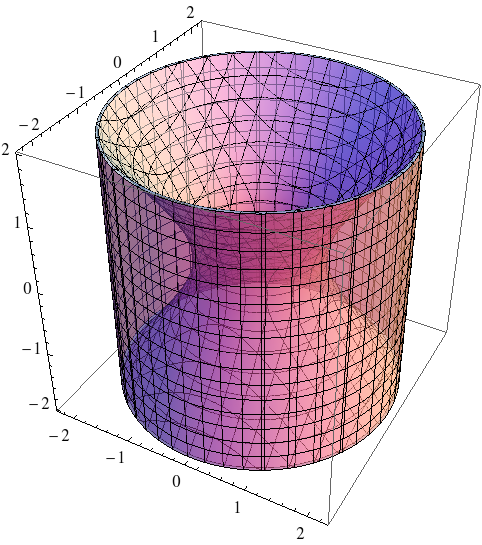
\includegraphics[scale=0.3]{Fig2.png}  
	\caption{Regi\~{a}o $ D_{xyz} = \lbrace(x, y, z)\mid x^2 + y^2 \geq 1 + z^2 $ e $ x^2 + y^2 \leq 5 \rbrace $}
	\label{fig:figura2}
\end{figure}

Realizamos a seguinte mudança de coordenadas:
\begin{equation}
\left\{\begin{array}{ll}
x=\rho\cos\theta\\
y= \rho\sin\theta\\
z = z
\end{array}\right.
\label{eq:Q2_mudanca}
\end{equation}

\begin{equation}
J = \begin{Vmatrix}
\cos\theta & -\rho\sin\theta & 0 \\
\sin\theta & \rho\cos\theta & 0 \\
0 & 0 & 1 \\
\end{Vmatrix} = \rho
\label{eq:Q2_Jac}
\end{equation}

Aplicando \eqref{eq:Q2_mudanca} \`a equaç\~{a}o do hiperbolóide:
\begin{equation}
\rho^2 = 1 + z^2 = \sqrt{1 + z^2}
\label{eq:Q2_hiperboloide}
\end{equation}

Aplicando \eqref{eq:Q2_mudanca} \`a equaç\~{a}o do cilindro :
\begin{equation}
\rho^2 = 5 \therefore \rho = \sqrt{5}
\label{eq:Q2_cilindro}
\end{equation}

Encontrando os valores de $z$ em que ocorre a intersercção do elipsoide com cone elíptico ( \eqref{eq:Q2_hiperboloide}) em \eqref{eq:Q2_cilindro} ):

$$ 1 + z^2 = 5 \Rightarrow z^2 = 4 $$
\begin{equation}
\therefore z = \pm 2
\label{eq:Q2_limitesDeZ}
\end{equation} \

Assim podemos facilmente descrever $D$ em coordenadas cilíndricas. \\

Calculando a integral : \

$$ \iiint_{D_{xyz}}{1}\;dx\,dy\,dz  = \int\limits_{0}^{2\pi} \int\limits_{-2}^{2}  \int\limits_{\sqrt{1+z^2}}^{\sqrt{5}}  \rho \;d\rho\, dz\,d\theta $$

Como o sólido é simétrico em $z$:

$$ = 2\int\limits_{0}^{2\pi} \int\limits_{0}^{2}  \int\limits_{\sqrt{1+z^2}}^{\sqrt{5}}  \rho \;d\rho\, dz\,d\theta =  2\int\limits_{0}^{2\pi} \int\limits_{0}^{2}   \frac{\rho^2}{2} \Big|_{\sqrt{1+z^2}}^{\sqrt{5}}  \; dz\,d\theta = \int\limits_{0}^{2\pi} \int\limits_{0}^{2}   (4-z^2)  \; dz\,d\theta $$
$$ = \int\limits_{0}^{2\pi}    \Big(4z-\frac{z^3}{3}\Big)_{0}^{2}  \; d\theta = \frac{16}{3} \int\limits_{0}^{2\pi} d\theta = \frac{32\pi}{3} $$

\newpage

%%%%%%%%%%%%%%%%%%%%%%%%%%%%%%%%%%%%% Questão 3 %%%%%%%%%%%%%%%%%%%%%%%%%%%%%%%%%%%%%%%%%%%%%%%%

\textbf{Quest\~{a}o 3.} (1,5 pontos) Calcule a massa do arame cujo formato é o da curva dada 	pela intersecção do parabolóide  $z = x^2 + y^2$ e o plano $2y + z = 1$, sendo a densidade $\delta(x,y,z) = \sqrt{2+4x^2}$. \\

\textbf{Solução:}
\linebreak
Devemos calcular a integral
\begin{equation}
 \int_{\gamma}{\delta(x,y,z)}\;ds \
\label{eq:integral}
\end{equation}

\begin{figure}[h!]
	\centering
	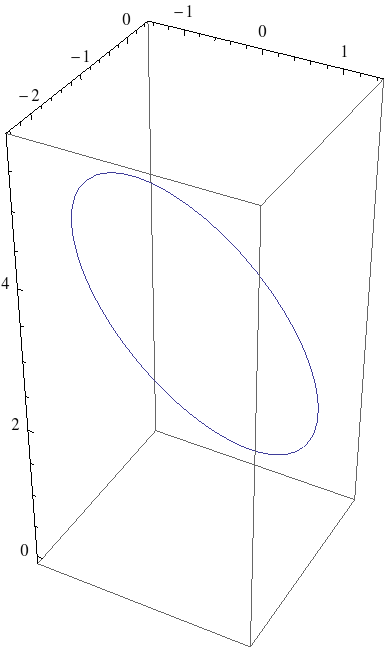
\includegraphics[scale=0.3]{Fig3.png}  
	\caption{Curva $\gamma(t)$}
	\label{fig:figura3}
\end{figure}

Parametrizando a curva em questão:

$$
\begin{cases}
z = x^2 + y^2 \\
2y + z = 1 \\
\end{cases}
\Rightarrow
\begin{cases}
z = 1 - 2y\\
1 - 2y = x^2 + y^2 \\
\end{cases}
\Rightarrow
\begin{cases}
z = 1 - 2y\\
 x^2 + (y+1)^2 = 2 \\
\end{cases}
\Rightarrow
\begin{cases}
x(t) = \sqrt{2}\cos t \\
y(t) = \sqrt{2}\sin t -1\\
z(t) = 3 - 2\sqrt{2}\sin t \\
\end{cases}
$$

\begin{equation}
\therefore \gamma(t) = (\sqrt{2}\cos t, \sqrt{2}\sin t -1, 3 - 2\sqrt{2}\sin t), t \in [0,2\pi]
\label{Q3_parametrizacao}
\end{equation}

$$ \gamma'(t) = (-\sqrt{2}\sin t, \sqrt{2}\cos t , - 2\sqrt{2}\cos t) $$
$$ ||\gamma'(t)|| = \sqrt{2 + 8\cos^2 t} $$ \\

Utilizando a definiç\~{a}o de integral de linha de uma função escalar:

$$  \int_{\gamma}{\delta(x,y,z)}\;ds = \int_{t_i}^{t_f} {\delta(\gamma(t)) ||\gamma'(t) ||}\;dt = \int_{0}^{2\pi} {\sqrt{2 + 8\cos^2 t} \sqrt{2 + 8\cos^2 t}}\;dt = \int_{0}^{2\pi} {2 + 8\cos^2 t}\;dt =  $$
$$ 2\int_{0}^{2\pi} dt + 8\int_{0}^{2\pi} {\frac{1+\cos 2t}{2}}\;dt = 4\pi + 4 \Big( t + \sin 2t \Big)_0^{2\pi} = 12\pi $$



\end{document}
